%%%%%%%%%%%%%%%%%%%%%%%%
% Sample use of the infthesis class to prepare an MSc thesis.
% This can be used as a template to produce your own thesis.
% Date: June 2019
%
%
% The first line specifies style options for taught MSc.
% You should add a final option specifying your degree.
% *Do not* change or add any other options.
%
% So, pick one of the following:
% \documentclass[msc,deptreport,adi]{infthesis}     % Adv Design Inf
 \documentclass[msc,deptreport,ai]{infthesis}      % AI
% \documentclass[msc,deptreport,cogsci]{infthesis}  % Cognitive Sci
% \documentclass[msc,deptreport,cs]{infthesis}      % Computer Sci
% \documentclass[msc,deptreport,cyber]{infthesis}   % Cyber Sec
% \documentclass[msc,deptreport,datasci]{infthesis} % Data Sci
% \documentclass[msc,deptreport,di]{infthesis}      % Design Inf
% \documentclass[msc,deptreport,inf]{infthesis}     % Informatics
%%%%%%%%%%%%%%%%%%%%%%%%

%\documentclass[msc,deptreport]{infthesis} % Do not change except to add your degree (see above).
\usepackage{yfonts}
\usepackage[pdftex]{graphicx}  
\usepackage{float}

\begin{document}
\begin{preliminary}

\title{Building a database to store Protein-Protein Interactions (PPI) in a rule based format}

\author{Ayush Das}

\abstract{
The study of Protein-Protein interactions (PPI) involves the analysis and identification of complexes that may form under a variety of reaction conditions. These reactions were initially modeled as Ordinary Differential Equations (ODEs) \cite{ode}, which is now progressing to a rule-based modeling approach. This is because the interacting biomolecules have the potential to interact in a myriad different ways. The number of possible post-translational modifications and complexes grow exponentially when considering the binary interactions within the reaction network. Using traditional methods like ODEs to model PPI requires large amounts of reaction specific details, and the chemical kinetics of the interactions within network requires explicit mention of the network conditions \cite{rule-based-general}. A rule-based model on the other hand comprises of, a set of rules where the network specification is implicit. These rules can specified using model specification languages like Kappa \cite{kappa} or BioNetGen \cite{bioNetGen}. Software tools enable researchers to model these interactions using different objectives like deterministic or stochastic modeling. Hence, researchers in bioinformatics have spent tremendous efforts in collecting the Protein-Protein interaction rules and the purpose of this project is to create and load a database with the PPI rules stored in a rule-based format. This will enable researchers to readily access PPI rules which when fed to a  simulator will enable study of the protein interactions and draw conclusions based on their observations.

% Cite BioNetGen
% Cite Kappa
% Cite  ODE
% Cite the first paper
}

\maketitle

\section*{Acknowledgements}
I would like to thank my supervisor Oksana Sorokina for her continued guidance and support during all stages of this project. The insightful feedback and guidance helped in improving the project to a large extent. I would also like to thank, Anatoly Sorokin and Douglas Armstrong for their insightful feedback and support during the course of this project.

Finally, I would like to thank my family for their support and guidance.

\tableofcontents
\end{preliminary}


\chapter{Introduction}
Protein is an important component of the cells in the human body. It is an important component of bones, muscles, cartilage and so on. Decades of research in the field of biology have produced a vast repository of knowledge on individual protein molecules. Examples of such knowledge base include UniProt \cite{uniprot}. However, in order to further explore the relationships of complex molecular species it is imperative to understand the interactions that take place between them and their governing rules.

As per \cite{ppiDef} Protein-Protein Interactions (PPI) are defined as the physical contacts with molecular docking between the protein molecules that occur in a living organism or cell. PPI interactions play a vital role as they dictate cellular activities which are responsible for good health or diseases. Achieving an in-depth understanding of protein interactions will help researchers improve the existing quality of medicine and health care in general. According to \cite{ppimp} an important source for drug discovery is the study of PPI. This is also evident from the fact that, as per \cite{cancer} in recent times the study of PPI has gained momentum for research in the field of anti-cancer therapy. All these facts suggest the importance of PPI and it's applications. 

Known PPIs are stored in PPI repositories designed to be easily retrievable by the researchers based on the relevant search term. There have been several databases in the past that have tackled the problem of collecting the PPIs. Such databases are of different varieties, based on their method of organizing and structuring the data. These kinds of databases are covered in greater detail, in Chapter 2. 

PPI interactions are used to model the dynamics of protein complexes in the cell. Initially they were modeled as Ordinary Differential Equations (ODEs) \cite{ode}, which have now progressed to a rule-based approach due to their ease and succinctness of expression. Rule-based methods have several applications some of which are assessing the druggability of proteins \cite{proteinDruggability} and drug effect pathway analysis \cite{pathwayAnalysis}. These will be dealt in greater detail, in the background section. 

This project is aimed at creating a database for Protein-Protein interactions stored in the Kappa rule format \cite{kappa}. The database would allow the PPI interactions to be retrieved based on certain conditions that are elaborated in Chapter 3. Rule based simulation of protein interaction can either be performed based on Stochastic Simulation Algorithm (SSA) or using Ordinary differential equations \cite{chylek2014rule}. In this project feeding the Kappa rules, to a Kappa simulator will help in visualizing the interactions of protein molecules in the Kappa simulator(KaSim) \cite{kasim}. KaSim is an implementation, of an algorithm called continuous time Monte-Carlo (CTMC), which is created for systems based on rules. 

This work is divided into chapters and we present a brief summary of each of these chapters. Chapter 2 covers, the kinds of PPI database that exist in literature, followed by a description of the kappa rules which encapsulates their syntax and semantics. The application of rule-based methods are also further elaborated in Chapter 2. Chapter 3 covers, the work that has been undertaken. This section elucidates the methodology used to create the database, the python scripts used to extract the relevant information from the assimilation of data collected by researchers. This section also elaborates on the SQL stored procedures used to extract the PPI rules and the user interface for accessing those rules. Furthermore, this chapter elaborates on the steps for deploying the database scripts and the web application. In Chapter 4, the validation pipeline for the data within the database is defined concisely. In this chapter we retrieve some of the PPI rules and validate the result set with the provided data. Chapter 5 presents the conclusion with future improvements and proposal for work that can be extended from the project.
% In the intodouction we write about what is PPI and why is it Important, what motivates the study of PPI, How will the database be useful, what the PPI Rules encapsulate, applications. What the other sections are all about. total 4 pages
%The preliminary material of your report should contain:
%\begin{itemize}
%\item
%The title page.
%\item
%An abstract page.
%\item
%Optionally an acknowledgements page.
%\item
%The table of contents.
%\end{itemize}

%As in this example \texttt{skeleton.tex}, the above material should be
%included between:
%\begin{verbatim}
%\begin{preliminary}
%    ...
%\end{preliminary}
%\end{verbatim}
%This style file uses roman numeral page numbers for the preliminary material.

%The main content of the dissertation, starting with the first chapter,
%starts with page~1. \emph{\textbf{The main content must not go beyond page~40.}}

%The report then contains a bibliography and any appendices, which may go beyond
%page~40. The appendices are only for any supporting material that's important to
%go on record. However, you cannot assume markers of dissertations will read them.

%You may not change the dissertation format (e.g., reduce the font
%size, change the margins, or reduce the line spacing from the default
%1.5 spacing). Over length or incorrectly-formatted dissertations will
%not be accepted and you would have to modify your dissertation and
%resubmit.  You cannot assume we will check your submission before the
%final deadline and if it requires resubmission after the deadline to
%conform to the page and style requirements you will be subject to the
%usual late penalties based on your final submission time.

%\section{Using Sections}

%Divide your chapters into sub-parts as appropriate.

%\section{Citations}

%Citations (such as \cite{P1} or \cite{P2}) can be generated using
%\texttt{BibTeX}. For more advanced usage, the \texttt{natbib} package is
%recommended. You could also consider the newer \texttt{biblatex} system.

%These examples use a numerical citation style. You may also use
%(Author, Date) format if you prefer.

\chapter{Background}
Protein-Protein interactions play a vital role in the regular functioning of life processes. Hence the study of these interactions, plays a crucial role in improving our understanding of diseases and the life processes.

Historically, PPI interactions were modeled using ordinary differential equations (ODE) \cite{ode}. However, as per \cite{rule-based-general}, this traditional approach of modeling PPI through ODE had several limitations due to the following reasons.

\begin{itemize}
\item
The protein molecules can potentially interact in an exponential number of ways. 
\item
Due to the exponential number of possibilities only large reaction networks can capture them.
\item
This is a problem because traditional approaches like ODE require explicit network specification.
\end{itemize}

This problem is overcome by the use of local rules where the network specification is implicit. As a result the specification of the model concise. These rules can be specified using languages for model specification like Kappa \cite{kappa}  and BioNetGen\cite{bioNetGen}. Specialized software tools then enable researchers to visualize the PPI interactions.

In the following sub-sections we will first explore the kinds of Protein interaction databases, followed by a section that develops on the understanding of rule based specification of protein interactions. This is then followed by a section that deals with the motivation of constructing the rule based database system and application of protein interaction database in biology.

\section{Protein-Protein Interaction (PPI) Databases}
As per \cite{typesOfPPIdb}, the kinds of protein-protein interaction databases can be divided into three types.
\begin{itemize}
	\item
	\textbf{Pathway:} In such databases researchers and domain experts collect rules that are generally agreed upon by the scientific community. These rules are manually curated and cover a large domain of information like association with diseases, stoichiometry of reactions and so on. Due to the requirement of manual intervention and the aim to achieve a high accuracy, construction of such databases is a laborious process.\\ Examples of such databases include KEGG \cite{kegg} and Reactome \cite{reactome}.
	\item
	\textbf{Experimentally Verified: } Such databases contain an assimilation of the protein interaction rules that have been experimentally verified. In other words such databases contain experimentally observed (verified) PPI rules. The method of the rule organization and the amount of information carried varies from one database to another. \\Examples of such databases include IntAct \cite{intact} and BioGrid \cite{biogrid}.
	\item
	\textbf{Experimentally Verified or Computationally predicted: } Such databases contain PPI rules that are either experimentally observed or are computationally predicted. These rules however, do not involve any manual organization. The computationally obtained PPIs may contain false positives and hence, to improve the accuracy a confidence score is often attached to the rules. In addition to using computational methods to obtain PPI rules, Natural Language Processing and text mining methods are also used in order to extract PPI rules from research literature.\\  Examples of such databases include  STRING \cite{string} and GeneMANIA \cite{genemania}.
\end{itemize}

While the three types of databases mentioned above, serve as the primary categorization of PPI databases, there also exists categorization of PPI databases based on diseases, organisms of particular kind and so on.

According to \cite{typesOfPPIdb}, there are over hundreds of databases that aim to collect and store protein interactions. However, none of these databases capture the complexity of biological systems in it's entirety. These kinds of details include - temporal dependencies, spatial dependencies, protein variations and so on.

\section{Motivation for constructing the rule based database}
As per \cite{kappaPlatform}, historical approaches aimed at storing the protein interactions were done so, through the method of deterministic models , based on differential equations. These models aimed to capture a myriad of information like post-translational, structural information an so on. Such a vast domain of knowledge was susceptible to errors or missing values, which cast a doubt upon their accuracy, as per \cite{kappaPlatform}. Such models also had maintainability issues because besides being difficult to build, they were also difficult to be updated with the ever evolving knowledge base that dictate these protein interactions. The human understanding of protein interactions matures and evolves with time and further research. Hence it is imperative to have a method of expressing PPI rules and building PPI models that make it easy to be read, stored and retrieved. As per \cite{kappaPlatform}, kappa rules, used to express the PPI interactions have the ability to encode and express information about the protein molecules (agents) and the sites that take part in the reaction. These rule summarize the pre and post conditions of the protein interaction without venturing into a detailed version of their structural analysis. Hence the rule based format of expressing PPI interaction is more concise. The stochastic models built using Kappa rules enable the description of complex interactions.

Hence, with this motivation in mind we have ventured to create a database of Protein-Protein interactions stored in a rule based format. The database created also has stored procedure routines that enable extraction of PPI rules based on certain conditions like agent name and domain name. The stored procedures are accessible via a web application built in django, with a user interface (UI), that enables the extracted rules to be printed or exported as CSV or Excel files. These files can be further analyzed and processed, fed to the kappa simulator \cite{kasim} and generate visualizations of the protein interactions.
\section{Understanding rule based specification of protein interactions}
\subsection{General Understanding of rule based languages}
In rule based languages like kappa \cite{kappa} and BioNetGen \cite{bioNetGen}, the agent is a conceptualization of the protein molecule. The protein molecules (agents) connect to form site graphs via the protein sites. The PPI rule as per the rule based format consists of a left hand denoted by $L_r$  side and a right hand side denoted by $R_r$. The $L_r$ and $R_r$ contain the site graphs which mention only the necessary sites for the protein interaction $L_r \to R_r$. 

Furthermore, \textswab{M} denotes the state of a system which is also called the reaction mixture. Each disconnected graph denotes one molecular species and the state of the system \textswab{M},  is a collection of disconnected graphs. The execution of a certain rule `r' implies the replacement of the mixture matched to $L_r$, with $R_r$, as shown in the Figure \ref{fig:mixture}. A model as per \cite{kappaPlatform} a collection of rules. Reasoning at the level of rules helps to introduce a level of compactness essential for the succinct expression of the protein interaction. 

\begin{figure}[H]
	\centering
	\captionsetup{justification=centering}
	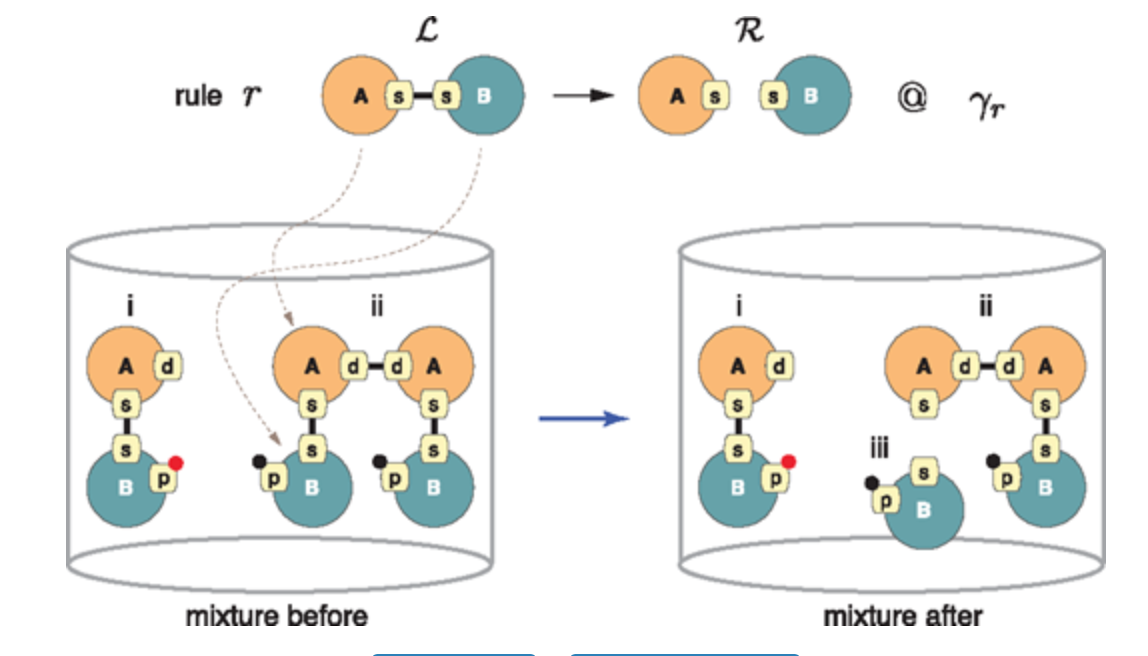
\includegraphics[width=\linewidth,height=10cm,keepaspectratio]{mixture.png}	
	\caption{Application of rule `r' to a reaction mixture \textswab{M} , comprising of two agents. $L_r$ and $R_r$ represent the state of the site graph before and after the application of rule `r'  respectively. Source: \cite{kappaPlatform}}
	\label{fig:mixture}
\end{figure}

Modeling tools built using latest technology help to visualize the protein interactions. Some examples of this include Virtual Cell \cite{vcell} and Kappa Simulator KaSim \cite{kasim}, which provide an environment for the modeling and simulation of cellular interactions. The Kappa rules can be fed into KaSim, which is a protein interaction simulator that implements continuous time Monte–Carlo algorithm (CTMC). KaSim  employs the process of stochastic modeling that can be used to describe highly complex interactions. Besides KaSim there also exist other stochastic modeling tools like STOCHSIM \cite{stochsim}, which can be used by researchers, to comapare the results.

\subsection{Syntax and semantics of Kappa rules}

\section{Application of Protein Interaction Database}
 

\chapter{Method}

A dissertation usually contains several chapters.

\chapter{Results and Discussion}

\chapter{Conclusions}

\section{Final Reminder}

The body of your dissertation, before the references and any appendices,
\emph{must} finish by page~40. The introduction, after preliminary material,
should have started on page~1.

You may not change the dissertation format (e.g., reduce the font
size, change the margins, or reduce the line spacing from the default
1.5 spacing). Over length or incorrectly-formatted dissertations will
not be accepted and you would have to modify your dissertation and
resubmit.  You cannot assume we will check your submission before the
final deadline and if it requires resubmission after the deadline to
conform to the page and style requirements you will be subject to the
usual late penalties based on your final submission time.

\bibliographystyle{plain}
\bibliography{mybibfile}

%% You can include appendices like this:
% \appendix
% 
% \chapter{First appendix}
% 
% \section{First section}
% 
% Markers do not have to consider appendices. Make sure that your contributions
% are made clear in the main body of the dissertation (within the page limit).

\end{document}
